\documentclass[a4paper,10pt,fullpage]{article}
\pagestyle{plain}
\usepackage[xdvi]{graphicx}
\usepackage{amsmath}
%\usepackage{times}
\usepackage{natbib}

\linespread{1.0}


\begin{document}
\begin{titlepage}

\flushleft

{\Large \bf LDhat 2.1: A package for the population genetic analysis
of recombination\\}

\vspace{1.5cm} {\it Gil McVean and Adam Auton\\}
mcvean@stats.ox.ac.uk\\
\begin{verbatim}
https://github.com/auton1/LDhat/
\end{verbatim}

\vspace{0.75cm}
Department of Statistics, Oxford, OX1 3TG, UK\\
\vspace{5.0cm}

Last updated: \today

\end{titlepage}

\tableofcontents

\newpage

\section{Introduction}
\verb+LDhat+ is a package of programs written in the C language for the
analysis of recombination from population genetic data.  The key
feature of the package is the estimation of population
recombination rates using the composite likelihood method of
Hudson \cite{Hudson01}, adapted to finite-sites models (applicable
to diverse genomes such as those of some viruses and bacteria)
\cite{McVeanetal02} and to estimate variable recombination rates
\cite{McVeanetal04, AutonMcVean07}. The method accommodates both phased or
haplotype and unphased or genotype data, with arbitrary levels of
missing data.

Within the package there are a number of programs.  Brief
descriptions of the programs are given below.

\begin{itemize}

\item {\bf convert}.  A simple manipulation program that
generates files in the appropriate format for subsequent analyses,
allows a number of options to be selected (e.g. minimum allele
frequency cutoff, missing-data cutoff, inclusion/exclusion of
sites with 3 or more alleles, data subsampling), and summarises
the input data. The files generated by the program are {\it
sites.txt}, which contains the sequence data, and {\it locs.txt}, which
contains the physical location of SNPs.

 \item {\bf pairwise}.  Estimates the population
recombination rate for the region analysed assuming a constant
recombination rate over the region and either a crossing-over or
gene conversion model. Takes as input the {\it sites} and {\it
locs} files generated by convert (or the user) and (usually) a
lookup table for the appropriate number of sequences, theta per
site, and grid size. For haploid or phased data with no missing
information {\bf pairwise} will, if prompted, generate a minimal
lookup table within the program. This option allows efficient
analysis of small data sets. However, other options within the
program (such as conditional simulation - see below) require the
exhaustive lookup file generated by {\bf complete} or {\bf lkgen}.  The program also performs additional analyses of recombination including estimation of the minimum number of recombination events and testing for the presence of recombination using the likelihood permutation test (LPT) described in \cite{McVeanetal02}.

 \item {\bf interval}.  Estimates a variable recombination rate
using a Bayesian reversible-jump MCMC scheme \cite{Green95} under
the crossing-over model (only).  As for {\bf pairwise}, the {\it
sites}, {\it locs}, and lookup table files are required.  The method was first published in \cite{McVeanetal04} and is the method used to estimate genome-wide fine-scale genetic maps from the Perlegen\cite{Myersetal05} and HapMap data sets \cite{HapMap05, HapMap07}.

\item {\bf rhomap}.  As with {\bf interval}, {\bf rhomap} estimates a variable recombination rate using a Bayesian reversible-jump MCMC scheme.  However, {\bf rhomap} specifically fits a model with recombination hotspots on a background of low rate variation.  In addition, the method rescales (flattens) the composite likelihood to improve estimation of posterior probabilities.  The method is described in \cite{AutonMcVean07}.

\item {\bf stat}.  Summarises the output from {\bf interval}. 

\item {\bf complete}.  Generates a lookup table required for all
analyses (except under certain circumstances, see {\bf pairwise}).
Input number of sequences, theta per site (assumes a two-allele
symmetric mutation model), and the grid size for $4N_er$ (in terms
of maximum value and number of points in the grid).  The program
calculates the coalescent likelihood of all possible two-locus
haplotype configurations using the importance sampling method of
Fearnhead and Donnelly \cite{FearnheadDonnelly01}.

\item {\bf lkgen}. Generate a lookup table from an existing one -
for a smaller number of sequences than the existing one, with the
same theta per site and grid size. Because of the computational
cost of calculating the lookup table, pre-computed tables for a
range of parameter values are available from
\verb+https://github.com/auton1/LDhat/+

\item {\bf fin}.  Coalescent simulation program to generate data sets for analysis with \verb+LDhat+.  The principal novelty of the program is that it enables simulation of arbitrary mutation models, however, it also includes standard options such as population growth, population bottlenecks, gene conversion and recombination hotspots.  It also includes an option to specify the positions and approximate allele frequencies of polymorphic sites.

\end{itemize}

\section{What's new in version 2.1?}

The two principal novelties in \verb+LDhat 2.1+ compared to \verb+LDhat 2.0+ are the inclusion of the {\bf rhomap} program \cite{AutonMcVean07} and the ability to specify all options on the command line.  The inclusion of the simulation program {\bf fin} is also novel.  In addition, there have been a few small bug fixes and improvement of data checking and error messages.  In addition, a series of R scripts are available for the analysis of program output from \verb+https://github.com/auton1/LDhat/blob/master/coalescent.r+.


\section{Installation}

The \verb+LDhat+ package is available as freeware from
\begin{verbatim}
https://github.com/auton1/LDhat
\end{verbatim}
\noindent C source code is provided for compilation using gcc on a Unix or Linux
operating system (or under a proprietary C compiler).  To install, move to the \verb+LDhat+ directory and type \verb+make+.  To remove
intermediate files, subsequently type \verb+make clean+.


\section{Input format}
The LDhat package accepts data in two formats: full sequence data,
or SNP surveys.  Full sequence data should be aligned and in a
modified FASTA format, with the first line detailing the number of
sequences/genotypes, the number of sites in the alignment and a
flag (1 or 2) that details whether the data is haplotype/phased
(1) or genotype/unphased (2). If full sequence data is used, {\bf
convert} should be used to generate the {\it sites} and {\it locs}
files needed for subsequent analyses (these can be renamed).
Sequence names should be no longer than 30 characters long, and
data should have no more than 2000 characters per line (line
breaks should be used to break up larger data sets).

The alternative format is to input segregating positions only, in
which case two files (referred to as the {\verb+sites+} and {\verb+locs+} files) are required.  The format of the {\verb+sites+} file is
identical to that for the full-sequence format (see example
below).  The {\verb+locs+} file has on the first line the number of
SNPs (segregating sites), the total length of the region analysed,
and a flag (L or C) that details whether a model of crossing-over
or gene conversion is fitted (see \cite{McVeanetal02}).  Following
the header line, the file contains the relative or absolute
location of SNPs/segregating sites in increasing order.  For large
SNP surveys it is recommended that positions are encoded in kb
rather than bp.

Haplotype/phased sequence data can either be coded in as standard
DNA letters (including ambiguous bases, N or ? for missing data
and - for gaps), or as 0/1/2/3.  For genotype/unphased data, the
convention used is 0 and 1 for the two homozygotes, and 2 for
heterozygotes.  For computational efficiency, all subsequent
analyses are restricted to those sites that have 2 alleles
segregating (i.e. monomorphic and sites with 3 or more alleles are
excluded). \\\\

\vspace{0.5cm}
\noindent Example {\verb+sites+} file format for haplotype full sequence data.
\begin{verbatim}
4  10  1
>SampleA
TCCGC??RTT
>SampleB
TACGC??GTA
>SampleC
TC?-CTTGTA
>SampleD
TCC-CTTGTT
\end{verbatim}
\vspace{0.5cm} \noindent Example {\verb+sites+} and {\verb+locs+} file
format for genotype data.
\begin{verbatim}
**Sites file**
 4 10 2
>GenotypeA
122110?000
>GenotypeB
1111201100
>GenotypeC
011111?112
>GenotypeD
2112210100

**locs file**
10  1200 L
1 57 180 187 223 250 438 509 878 1034
\end{verbatim}

\noindent An example data set, {\verb+lpl_fn.sites+} and {\verb+lpl_fn.locs+},
is included in the package.

\section{Using the programs}
This section provides a detailed description of the input and
output generated by each program and the options available within
them.  Where command-line arguments are given, arguments in square
parentheses indicate options.   Due to computational load, at
present there is a limit of 300 sequences that can be analysed
within the program.  If more sequences are included, only the
first 300 will be analysed.

All programs can be run from the command line.  However, if command line options are not specified, the user will be prompted for the relevant inputs by the program.  For each program a list of the options, along with a brief description, can be obtained by using the flag -h.  For example, \\
\begin{verbatim}
% ./convert -h 
\end{verbatim}
gives a list of the options that can be specified for the program {\bf convert}.  Note that if any command-line options are specified, all other options will be set at their defaults. In the following description, where the user has to input a parameter following the use of a particular flag the type of parameter is indicated within the symbols \verb+<>+.  For example,  \\
\begin{verbatim}
% ./convert -freqcut <float> 
\end{verbatim}
means that a floating point number has to follow the use of the \verb+-freqcut+ flag.


\subsection{convert}
To run {\bf convert} from the command line type\\
\begin{verbatim}
% ./convert -seq <file_name> 
\end{verbatim}
If no file is specified, the user is prompted for the input file
name within the program.  If the name of a {\it locs} file is also
included on the command-line, the program will use this to provide
the relative position of each SNP (this option cannot be accessed
from within the program), otherwise it is assumed that sites are
contiguous.

The program reads in the input file(s), and produces a summary
file {\verb+freqs.txt+} that details the frequency of each allele at
each site.  Options about output can be specified using command-line flags or if no command-line options are specified.

\begin{itemize}
\item \verb+-loc <file>+: Specify a file containing the position of  sites (in \verb+LDhat+ format).
\item \verb+-2only+: Specifies that only polymorphic sites with exactly two alleles will be analysed and outputted  Although
only those sites with two alleles are analysed in {\bf pairwise} and
{\bf interval}, outputting all segregating sites may be
of interest and can be used to estimate a finite-sites estimate of
Watterson's theta per site within {\bf pairwise} \cite{McVeanetal02}.  

\item \verb+-freqcut <double>+: The user
can specify a minimum minor allele frequency (MAF) cutoff (e.g.
\verb+-freqcut 0.2+ specifies those sites with a MAF$>20$\%). The default cutoff is 0 (i.e.all polymoprhic sites are outputted).  Note this option also means that only sites with exactly two alleles will be outputted.

\item \verb+-missfreqcut <double>+:  Frequency cut-off for missing data. Sites with large amounts
of missing data slow subsequent analyses. Specify the frequency of
missing data above which sites are excluded from subsequent
analyses (e.g. \verb+-missfreqcut 0.2+ specifies 20\%).  The default is 100\% (i.e. include all sites irrespective of missing data).

\item \verb+-sites <int> <int>+: Only print out sites between the specified positions.

\item \verb+-nout <int>+: Specify the number of sequences to output.  If this is less than the total number of sequences inputted, a random sub-sample is drawn.
 
\end{itemize}
\noindent The program ends by summarising the input data with four
statistics.  These are

\begin{itemize}
\item The number of segregating sites in the output file

\item The average pairwise differences (PWD) between sequences

\item Watterson's infinite-sites estimator of the
population-scaled mutation rate $\theta=4N_e\mu$ for diploid
species, or $\theta=2N_e\mu$ for haploid species.  Note that this
estimate applies to the whole region (i.e. is not per site), {\bf
pairwise} will also estimate a theta, but this is a {\it per site}
estimate based on a finite-sites approximation to Watterson's
estimate \cite{McVeanetal02}.

\item Tajima's D statistic \cite{Tajima89}.  A measure of
departure from neutral expectation.  Significance levels under the
assumption of no recombination can be found in Tajima's paper
\cite{Tajima89}. Significance levels with recombination can be
estimated by Monte-Carlo simulation, e.g. using Hudson's
makesamples program \cite{Hudson02}, or DNAsp \cite{Rozasetal03}.

\item Fu and Li's D* statistic \cite{FuLi93}.  Another summary of
the departure of the frequency spectrum from neutral expectations,
that focuses on the number of singletons (sites at which only a
single sequence differs from the rest of the sample).

\end{itemize}

\noindent The program generates two files, {\verb+sites.txt+} and {\verb+locs.txt+}, which may be renamed and used in subsequent analyses. These
contain the data at the sites selected and the position of the
sites.

\subsection{pairwise}
Performs estimation of the population-scaled recombination rate
$\rho=4N_er$ for diploid species, or $\rho=2N_er$ for haploid
species, where $N_e$ is the effective population size and $r$ is
the genetic map distance across the region analysed (the product
of the physical distance and the per site rate of recombination
across the region).  The composite likelihood method of Hudson
\cite{Hudson01} is used, although in contrast to Hudson, a
finite-sites model is used to estimate the coalescent likelihood
of two-locus haplotype configurations \cite{McVeanetal02}.  The
use of a finite-sites model enables the use of the
composite-likelihood method in species, such as viruses and
bacteria, where sites may have experienced multiple mutations in
the history of the sample; see McVean et al. \cite{McVeanetal02}
for more details.  It should be noted that the model also assumes
uniformity of the mutation rate across sites. Extreme rate
heterogeneity can cause homoplasy that mimics the effects of
recombination.  For this reason, in highly diverse genomes,
analysis of codon positions 1 and 2 apart from position 3 is
recommended.  However, the nonparametric tests employed in the
program to test the hypothesis of no recombination are robust to
rate heterogeneity and complex mutation models
\cite{McVeanetal02}.

To run the program from the command line type

\begin{verbatim}
% ./pairwise -seq <file_name> -loc <file_name>
\end{verbatim}
If no file-names are specified, the user will be prompted within
the program.  If no lookup table is available, one specific to the
data set will be generated within the program. Flags and analyses available witihn the program are described below.  Note that this program is not currently totally command-line driven - the user will be asked for some options within the program.

\begin{itemize}
\item \verb+-lk <file_name>+: Specify the use of a pre-calculated lookup table.  If specified, the
name of the lookup table should be inputted followed by whether
the lookup table is exact specified by option \verb+-exact+ (exact means specific to the data set, including
missing data and unphased/genotype information). If no lookup table is specified, the program will ask the user to input parameters to
estimate the lookup table specific to the data (note that this option will not work if the data contains missing information or it is unphased genotype data).  In order, these
are: A) The theta per site to use (with a suggestion made from the
finite-sites version of Watterson's estimate); B) The maximum
value of $4N_er$ (equivalent to $2N_er$ for haploid organisms) for
the grid, with a suggested value of 100; and C) The number of
points on the grid (with a suggestion of 101).  The choice of
parameters for the grid (which is uniformly spaced) specifies the
accuracy and computational load of the calculation; large values
for the maximum $4N_er$ and points will take longer and give more
accurate results.  However, it is suggested that the max $4N_er$
value should be in the range 20-100 (values greater than 100 are
treated as 100), and the number of points should be in the range
21-201.  The estimation of the lookup table may take up to a day
on a standard desktop.  It is therefore recommended that wherever
possible existing lookup tables that include all possible
two-locus haplotype configurations are used or generated from
existing ones (see {\bf lkgen}).  Furthermore, for
unphased/genotype data, and data sets with missing data, such an
exhaustive lookup table is required. It is worth noting that minor
changes in the value of theta per site used do not seem to have a
large influence on the estimated recombination rate.

\item Estimation of the recombination rate.  Once the lookup table
has been generated/read in, the user will be prompted for whether
to change the default values for the grid over which the
population recombination rate (for the whole region) should be
changed (option 1 = yes, option 0 = no).  Initially, the defaults
should be accepted, but if the estimated value is at the extreme
of the grid, subsequent analyses should change the defaults. If
the grid over which likelihoods have been calculated is large and
fine (e.g. max $4N_er = 100$, no. points = 101), there is no
restriction in estimating rates over the region analysed which
extend into the 1000s.  If possible, it is worth having in mind a
rough figure for the value you expect over the region.  Generates
a file {\verb+outfile.txt+}.

\item Calculating fits (no user prompting - see below for
details).  Generates a file {\verb+fits.txt+}.

\item Sliding windows analyses.  An equivalent estimation
procedure can be carried out in a sliding-windows fashion to look
at recombination rate variation in the region (though this
analysis is largely superseded by {\bf interval} (see below).  If
this option is selected (option 1), the user is prompted for the
number and length of the windows (the degree of overlapping is
determined by these options).  Generates a file {\verb+window_out.txt+}.

\item Rmin values.  Uses Hudson and Kaplan's estimator of the
minimum number of recombination events \cite{HudsonKaplan85} to
describe the evidence for recombination across the region.  Option
1 simply prints to screen the minimum over the region (which is a
lower bound on the true minimum in the infinite-sites model).
Option 2 prints both the total, but also generates a file {\verb+rmin.txt+}, which details the estimated minimum between all pairs
of SNPs using the dynamic programming algorithm of Myers and
Griffiths \cite{MyersGriffiths03}.

\item Moment method.  Uses Wakeley's \cite{Wakeley97} adaptation
of Hudson's \cite{Hudson87} moment method to estimate the
population-scaled recombination rate across the region from the
variance in the pairwise differences between sequences.

\item Test for recombination.  Nonparametric permutation tests for
the influence of recombination.  The distribution of four
statistics of the data (maximum composite likelihood, summed
difference between all pairs of sites that show evidence of
recombination by the four-gamete test, correlation between the
$r^2$ measure of linkage disequilibrium (LD) and physical distance
and correlation between the $|D'|$ measure of LD and physical
distance) are calculated under random permutation of the physical
position of the SNPs (1000 permutations).  The values observed in
the unpermuted data are compared to these null distributions to
describe the evidence for a non-zero rate of recombination.  The
power and properties of these tests are described in
\cite{McVeanetal02}.  Currently, these tests are only available
for phased/haplotype data.  Generates a file {\verb+rdist.txt+}.

\item Parametric simulation.  Monte Carlo coalescent simulations
are carried out using the estimated population recombination rate
and the inputted value of theta per site, which condition on the
location and approximate allele frequency of SNPs in the sampled
data.  These simulations are used to generate the sampling
distribution of the point estimate of the population-scaled
recombination rate and to test the hypothesis of a constant
recombination rate over the region.  If simulations are to be
performed, an exhaustive lookup table must be used. Currently only
available for phased/haplotype data. Generates a file {\verb+sim_out.txt+}.

\item flag \verb+-concise+: Suppress much of the output except for key results.
\end{itemize}

\noindent A brief description of the contents of the output files.
\begin{itemize}
\item {\verb+outfile.txt+} contains the point estimate of the
population recombination rate for the region and the composite
likelihood surface.  The likelihood surface for the sample data
set is shown in Figure \ref{fig:lpl_surf}.


\begin{figure}
\linespread{1.3} \centering
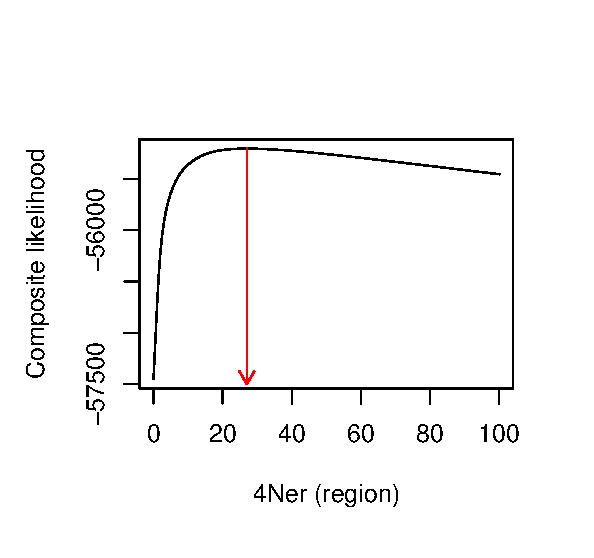
\includegraphics[scale=1.0]{LPLCLcurve.eps}
\caption{Composite-likelihood curve for the LPL data set from
Finnland (48 haplotypes) \cite{Nickersonetal98}.  The maximum
occurs at $4N_er=27$ for the 9.7~kb region} \label{fig:lpl_surf}
\end{figure}

\item {\verb+new_lk.txt+} contains the lookup table specific to the
data set.  This should be renamed and used in future analyses,
e.g. for {\bf interval}.

\item {\verb+fits.txt+} contains a upper-diagonal matrix with the
marginal likelihood-ratio test statistic for each pair of sites.
For each pair of SNPs, $i$ and $j$, the reported value represents
the difference in log composite-likelihood between the
best-fitting model that assumes a constant recombination rate over
the entire region, and the marginal maximum for the pair of sites.
For example, suppose there is a 1kb region for which the maximum
composite likelihood for the entire data is achieved at $4N_er =
100$.  A pair of SNPs at 250bp and 750bp would therefore have a
recombination distance of $4N_er = 50$, but if we were looking at
just those sites, maybe the likelihood would be maximised at
$4N_er = 10$.  The difference in log likelihood between these
estimates is then reported, multiplied by $+1$ if the marginal
maximum is achieved at a higher $4N_er$ than the estimated value
or $-1$ if the marginal maximum is achieved at a lower $4N_er$
than the estimated value.  Also calculated is the sum of the
composite log likelihood ratio test statistics across pairs.  The
matrix can be used to visualise the discordance between the fitted
(constant) rate patterns in the data; see Figure
\ref{fig:lpl_fit}.

\begin{figure}
\linespread{1.3} \centering
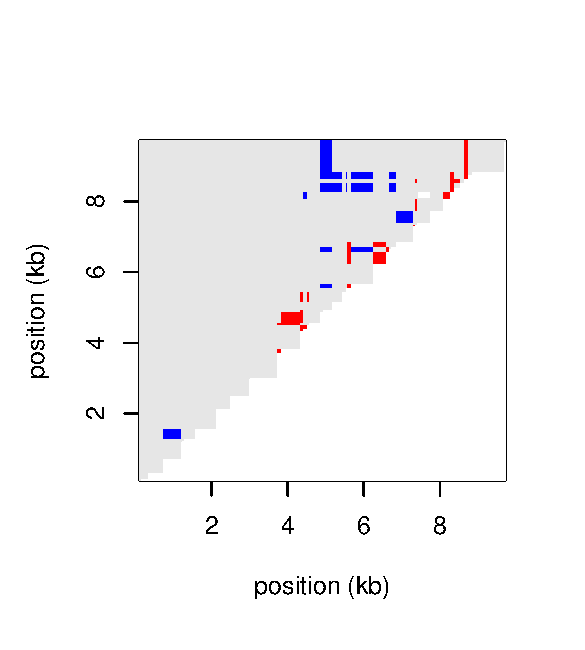
\includegraphics[scale=1.0]{LPLfit.eps}
\caption{For the LPL data, a plot showing which pairs of sites
have unusual patterns of LD given the assumption of a constant
recombination rate.  Pairs with a marginal likelihood ratio
greater than 2.0 are coloured (red for pairs with less LD than
expected, blue for pairs with more LD than expected, gray for
other pairs). The block of red in the centre suggests the presence
of a recombination hotspot} \label{fig:lpl_fit}
\end{figure}

\item {\verb+window_out.txt+} contains the output of the
sliding-window analysis.  The columns are (in order):  the
position of the left-most SNP in the window, the position of the
right-most SNP in the window, the number of SNPs in the window,
the window estimate of the recombination rate per bp or kb
(depending on whether the {\verb+locs+} file is in bp or kb), the log
composite likelihood ratio comparing the locally estimated rate to
the rate estimated for the whole region, and Tajima's D statistic
for the window.  The log composite likelihood ratio is an
indicator of the degree to which the window differs from the
region as a whole, but should not be used as a standard likelihood
ratio test statistic.

\item {\verb+rmin.txt+} contains the output from the Rmin analysis.
For each pair of sites $i$ and $j$ ($j>i$), the upper diagonal
element $(i,j)$ is the minimum number of recombination events that
occurred in the history of the sample between these positions, and
the lower diagonal element $(j,i)$ is that value divided by the
physical distance between the SNPs.  This matrix can also be used
to derive graphical representations of the extent of recombination
in the sequence, see Figure \ref{fig:lpl_rmin}.

\begin{figure}
\linespread{1.3} \centering
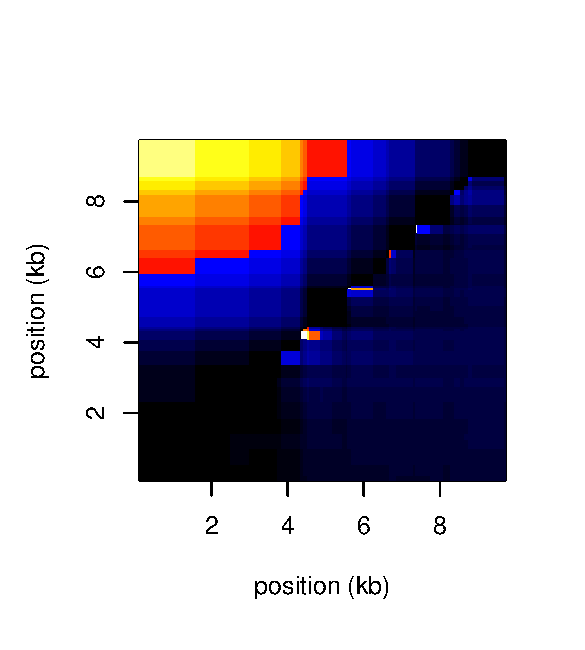
\includegraphics[scale=1.0]{LPLrmin.eps}
\caption{Detectable recombination events in the LPL gene (Finnish
population) using the method of Hudson and Kaplan
\cite{HudsonKaplan85}.  Above the diagonal, values represent the
minimum number of detected recombination events between pairs of
sites. Below the diagonal, the minimum number of recombination
events is rescaled by the physical distance between pairs of sites
to represent the local intensity of recombination.  The cluster of
recombination events in the centre of the gene again suggest a
recombination hotspot} \label{fig:lpl_rmin}
\end{figure}

\item {\verb+rdist.txt+} contains the results of the permutation
analyses designed to test for the presence of recombination. These
data can be used to compare the distribution of the test statistic
against the observed value.

\item {\verb+sim_out.txt+} contains details of the parametric
simulations carried out to test for recombination-rate uniformity
and calculate the sampling distribution of the point-estimate of
the recombination rate.  The columns in the file are respectively,
the point estimate of rho from the simulation, the summed marginal
log composite likelihood test statistics across pairs of SNPs (see
above), the difference in log composite-likelihood between the
maximum and that obtained at the value the data was simulated
under (for assessing the null distribution of the log composite
likelihood ratio test statistic), and a correction factor (CF),
which is proportional to the log of the probability of the
simulated data under the coalescent model.  The final column could
be used to weight simulations, however the test is carried out in
the manner of Hudson \cite{Hudson93}, where all simulations are
given equal weight.

\end{itemize}



\subsection{interval}
Performs estimation of variable recombination rates using a
penalised likelihood within a Bayesian reversible-jump Markov
chain Monte Carlo scheme (rjMCMC) as described in \cite{McVeanetal04}.  Note, however, that because of
the assumptions introduced by the use of composite-likelihood, the
standard Bayesian interpretation of the output of the chain cannot
be said to represent the posterior distribution of rate estimates.
Rather, a summary of the output should be used to describe the
analysis of the data, and comparison to simulations should be used
to draw statistical inferences; see \cite{McVeanetal04} for
details of the method.

The program requires the same input files as {\bf pairwise},
except that a lookup table is essential.  To run it from the
command line, type\\
\begin{verbatim}
% ./interval -seq <file_name> -loc <file_name> -lk <file_name> 
\end{verbatim}
If no file-names are specified, the user will be prompted within
the program.   The various options and flags are described below
\begin{itemize}

\item \verb+-seq <file_name>+: Name of file containing sites.

\item \verb+-loc <file_name>+: Name of file containing positions of polymorphic sites.

\item \verb+-lk <file_name>+: Name of file containing lookup table.

\item \verb+-exact+:   As with {\bf pairwise} lookup
tables can either be exhaustive (i.e. contain every possible
two-locus haplotype configuration with no missing data for the
number of sequences as generated by {\bf complete} or {\bf
lkgen}), or exact (contain all two-locus configurations for the
specific data set including missing-data and genotype data), as
generated by {\bf pairwise}.  If the flag is not included it will be assumed that the lookup table is exhaustive.

\item \verb+-its <int>+: Number of iterations for the rjMCMC procedure.  It is recommended to use a minumum of 1,000,000, but 10x more will give more consistent results.  If this is not specified on the command line, the user will be prompted later.


\item \verb+-bpen <float>+: Block penalty.  The method works by fitting a piece-wise
constant recombination rate to the data, where changes in rate can
only occur at SNPs.  To avoid over-fitting, a penalty is
introduced, which is multiplied by the number of change-points in
the estimate genetic map and added to the log composite
likelihood.  Large penalties identify positions at which there is
very strong evidence for changes in recombination rate, but will
loose detail.  Small penalties reveal detail, but also introduce
noise.  Calibration of the method by simulation has shown that a
penalty of 5 is adequate for the analysis of large data sets in
humans (also the value used in the analysis of the HapMap \cite{HapMap05, HapMap07} and Perlegen \cite{Myersetal05} data sets), but it is recommended that the user uses a series of
penalties in the range 0-50.  Monte Carlo simulations can
potentially be performed 
to assess the performance of the method under different
conditions; see \cite{McVeanetal04} for full details.

\item \verb+-samp <int>+: Number of updates between samples.  For efficiency, it is
often preferable not to keep the results from every iteration of
the Markov chain.  It is recommended that sampling every 2000-5000
iterations is adequate.


\end{itemize}

\noindent  Once initiated, the Markov chain is left to run.  At
each sample, a summary is printed to screen that details the
iteration number, the current likelihood of the data (excluding
change-point penalties), the number of blocks with uniform
recombination rate (the number of change points plus one) and the
total population recombination rate over the region analysed (map
length).  Efficient mixing of the algorithm can be observed if the
summaries change frequently.

Two files are generated as the Markov Chain progresses.  {\verb+rates.txt+} is the output from each sample detailing the
recombination rate (expressed in $4N_er$ per kb or bp depending on
the format of the {\verb+locs+} file) between each SNP.  {\verb+bounds.txt+} details
the position of the change points along the sequence at each
sample.  The program {\bf stat} should be used to summarise these
two files.

At the end of the run, acceptance rates for each of the proposed
moves in the rjMCMC scheme are detailed.  Because of the
composite-likelihood scheme, these rates are often very low (of
the order of 1\% or less), indicating that the chain needs to be
run for a long period of time for appropriate sampling.

Also generated is a file {\verb+new_lk.txt+}.  As for {\bf
pairwise}, this file should be renamed and used in future analyses
with {\bf interval} as an exact lookup table.  Note however, that
this file cannot be used for {\bf pairwise}.

An example of the output from \verb+interval+ for the LPL data is shown in Figure \ref{fig:lpl_interval}.




\begin{figure}
\linespread{1.3} \centering
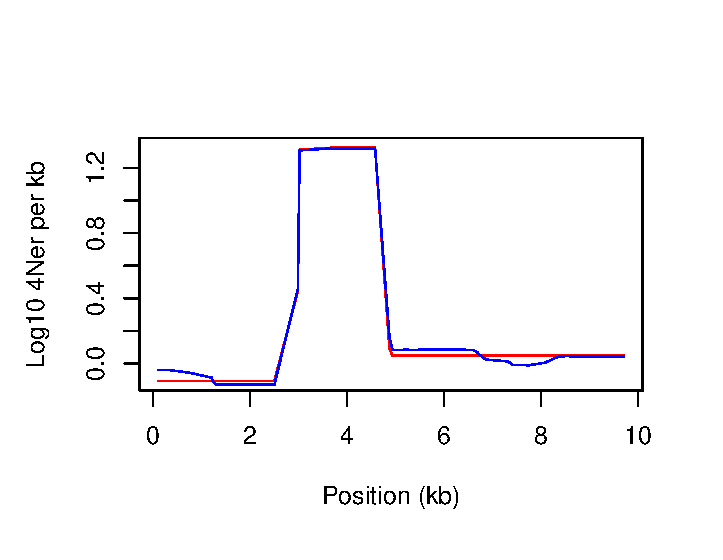
\includegraphics[scale=1.0]{LPLinterval.eps}
\caption{The estimated recombination rate across the LPL gene from
the Finnish sample for penalties of 5 (blue) and 20 (red). The
point estimate of the rate is given by the average rate from the
posterior} \label{fig:lpl_interval}
\end{figure}


\subsection{rhomap}

{\bf rhomap} is an extension of the algorithm used in {\bf interval} in which hotspots are explcitly modelled.  See \cite{AutonMcVean07} for details.  The input and output are similar to that of {\bf interval}.   There are two key differences with {\bf interval}.  First, in addition to background rate variation, hotspots (modelled with a specific form) are also included, which have a location, a heat and a width.  Second, the composite likelihood is 'flattened' by a factor to resemble a true likelihood.  The scaling factor is set such that under a model of fee recombination the composite likelihood returns the true likelihood.  For low recombination rates, the likelihood surface wlil tend to be over-flattened.  

The model employed in {\bf rhomap} is specifically aimed for analysing human data and will perform better than {\bf interval} in estimating recombination rates when the true underlying profile includes sharply-peaked recombination hotspots.  It is possible to alter parameters for any species, but we suggest that extensive simulations should be carried out using appropriate SNP densities, hotspot densities and intensities and background rate levels to find appropriate parameters.  We also suggest that other methods, such as \verb+LDhot+ \cite{McVeanetal04, Myersetal05} or \verb+SequenceLDhot+ \cite{Fearnhead06}, are used if the goal of the analysis is specifically to identify recombinaton hotspots.  


To run it from the
command line, type\\
\begin{verbatim}
% ./rhomap -seq <file_name> -loc <file_name> -lk <file_name> 
\end{verbatim}
If no file-names are specified, the user will be prompted within
the program.   The various options and flags are described below
\begin{itemize}

\item \verb+-seq <file_name>+: Name of file containing sites.

\item \verb+-loc <file_name>+: Name of file containing positions of polymorphic sites.  Note that this is assumed to be in kb (i.e. position 1,234 should be written as 1.234).

\item \verb+-lk <file_name>+: Name of file containing lookup table.

\item \verb+-its <int>+: Number of iterations for rjMCMC.

\item \verb+-samp <int>+: Number of iterations between successive samples from the chain.

\item \verb+-burn <int>+: Number of iterations to run chain for as burn-in period (i.e. before sampling begins).

\item \verb+-exact+: Indicates that the lookup table specified is exact (see {\bf pairwise} or {\bf interval} for a definition of exact).  

\item \verb+-seed <int>+: User-defined seed for random-number generator.

\item \verb+-no_files+: Do not output MCMC samples.

\item \verb+-fileprefix <string>+: Prefix for naming ALL output files.

\end{itemize}

The model with hotspots is characterised by several parameters and hyperparameters that can either be left at their default settings or changed by the user (see \cite{AutonMcVean07} for a discussion of relevant values).  Default values can be found in the file \verb+params.h+ in the source code.  The parameters are

\begin{itemize}

\item \verb+-bpen <float>+: Penalty for change points in background rate (default = 0).

\item \verb+-hpen <float>+: Penalty for hotspot (default = 0).

\item \verb+-bgAlpha <float>+:          Background rate prior alpha (Gamma Distribution)
\item \verb+-bgBeta <float>+:           Background rate prior beta (Gamma Distribution)
\item \verb+-HeatAlpha <float>+:        Hotspot heat prior alpha (Gamma Distribution)
\item \verb+-HeatBeta <float>+:         Hotspot heat prior beta (Gamma Distribution)
\item \verb+-ScaleAlpha <float>+:       Hotspot scale prior alpha (Gamma Distribution)
\item \verb+-ScaleBeta <float>+:        Hotspot scale prior beta (Gamma Distribution)
\item \verb+-T <float>+:                Expected Hotspot seperation (default = 50kb).
\item \verb+-m <float>+:                Maximum extent of hotspots (default = 5kb)

\end{itemize}



\noindent  Once initiated, the Markov chain is left to run.  At
each sample, a summary is printed to screen that details the
iteration number, the current likelihood of the data (excluding
change-point penalties), the number of changepoints in the background recombination rate, the number of hotspots and the total map length.  Efficient mixing of the algorithm can be observed if the
summaries change frequently.

Four files are generated as the Markov Chain progresses.  {\verb+acceptance_rates.txt+} details the acceptance rates.  {\verb+hotspots.txt+} contains details of the hotspots at each sample from the chain.  {\verb+rates.txt+} is the output from each sample detailing the
recombination rate (expressed in $4N_er$ per kb) between each SNP. {\verb+summary.txt+} contains a summary of the samples from the chain detailing, for each SNP interval, the estimated genetic map position, the estimated recombination rate, and the hotspot density (the number of hotspots per kb per iteration).  The {\verb+rates.txt+} file can be summarised by use of the program {\bf stat}.  Figure \ref{fig:lpl_rhomap} shows the estimated rate over the LPL gene from the Finnish sample using \verb+rhomap+.  





\subsection{stat}

Summarises the output from {\bf interval} in terms of the average,
median, 2.5th percentile and 97.5th percentile of the estimated
recombination rate between each pair of SNPs.  To run the program
from the command-line type\\
\begin{verbatim}
% ./stat -input <file_name>
\end{verbatim}
If no file is specified, the user will be asked to input the file
name.  Files should be of the format of {\it rates.txt} and {\it
bounds.txt}, with the first line detailing the number of samples
and the number of elements at each sample.  The burn-in specifies
the number of entries to be ignored in the summary.  It is
recommended that the first 100,000 iterations of the rjMCMC scheme
are excluded.  The output file, {\it res.txt}, is a summary of the
samples from the rjMCMC chain. An example of the summary is shown
in Figure \ref{fig:lpl_interval} for two different values of the
penalty (5 and 20). Note that the first entry in the {\it
rates.txt} file corresponds to the total population genetic
distance across the region (the map length).  Visual inspection of
the estimates from the rjMCMC should be used to check for
convergence, along with multiple runs starting from different
points (see Figure \ref{fig:lpl_samples}).  Stat has only one option.

\begin{itemize}
\item \verb+-burn <int>+: Specify the number of samples to be discarded as burn-in.
\end{itemize}

The estimated recombination rate across the LPL gene from
the Finnish sample using {\verb+rhomap+} with both background and hotspot penalties of 0. The
point estimate of the rate is given by the average rate from the posterior.

\begin{figure}
\linespread{1.3} \centering
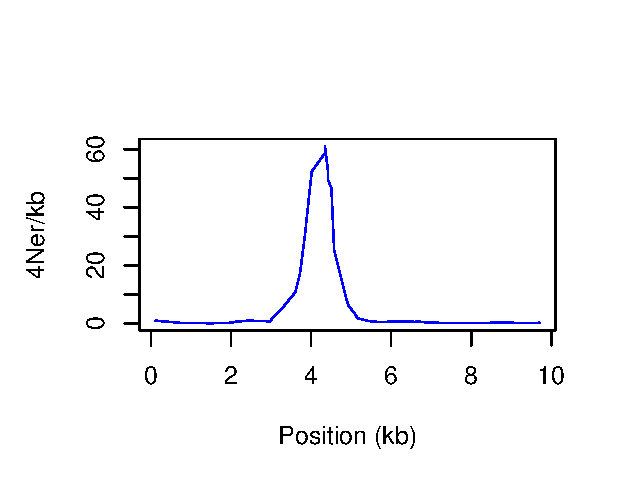
\includegraphics[scale=1.0]{lpl_rhomap.eps}
\caption{The estimated recombination rate across the LPL gene from the Finnish sample estimated with rhomap (both hotspot and background penalties set to 0)}
\label{fig:lpl_rhomap}
\end{figure}

\begin{figure}
\linespread{1.3} \centering
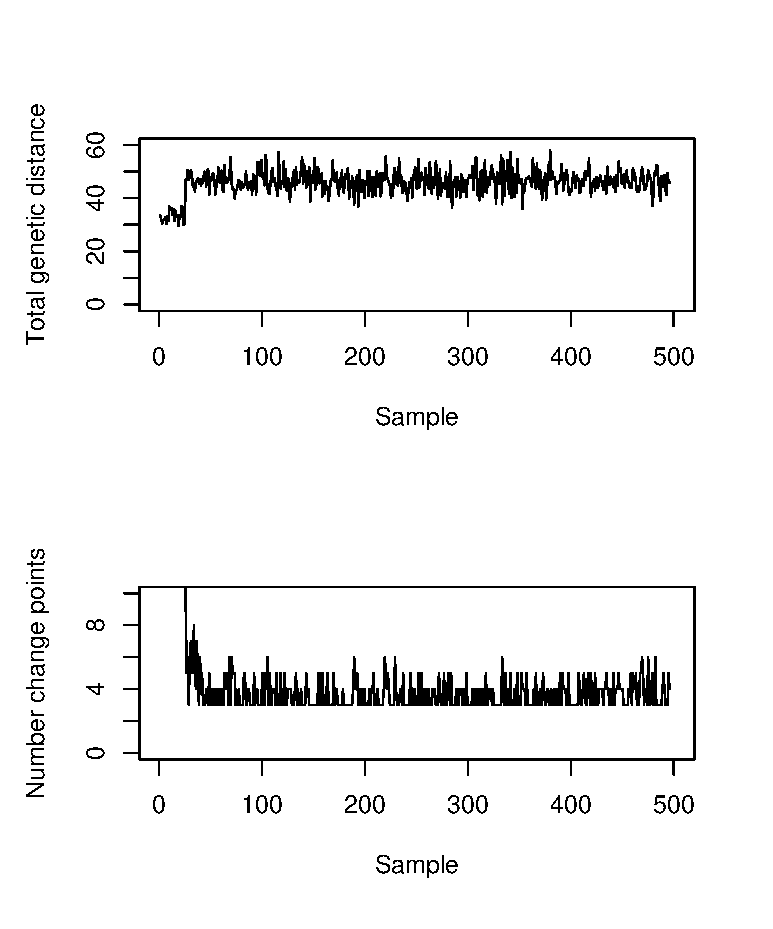
\includegraphics[scale=1.0]{LPLsamples.eps}
\caption{Samples from the RJMCMC for the Finnish LPL data with a
penalty of 20. The top panel shows the total genetic distance over
the region over a short run of 1000000 updates.  For the same run,
the lower panel shows the number of change points at each sample
(taken every 2000 updates)} \label{fig:lpl_samples}
\end{figure}


\subsection{complete}
Generates a lookup table with the coalescent likelihoods for every
possible two-locus haplotype configuration for a given sample
size, using a user-defined theta per site and a grid of
recombination rate values.  The importance sampling method of
Fearnhead and Donnelly \cite{FearnheadDonnelly01} is used.  Note,
that because the importance sampling method is Monte-Carlo (i.e.
simulation-based), different runs of the program may give very
slightly different results.  To use the program, type (at the command-line)
\begin{verbatim}
% ./complete 
\end{verbatim}
The  options are
\begin{itemize}
\item \verb+-n <int>+: The number of chromosomes (Note that if your data is diploid you will need to make a table for 2x the number of individuals).

\item \verb+-rhomax <float>+: The maximum value of $4N_er$ to estimate likelihoods for (the minumum is always 0).  It is suggested that this value should be 100.

\item \verb+-n_pts <int>+: The number of points in the grid (suggested to be 101).

\item \verb+-theta <float>+: The value of $\theta = 4N_eu$ per site.  A suitable estimate can be obtained by running {\bf pairwise} first.  

\item \verb+-split <int>+: Split the calculation into \verb+<int>+ blocks - useful, for example, if you wish to use a cluster to calculate the lookup table.  The flag \verb+-element <int>+ defines which of the elements to calculate the likelihood for.  For example, a lookup table for 50 sequences can be broken into 10 sections - to calculate the first of these sections type\\
\begin{verbatim}
./complete -n 50 -rhomax 100 -n_pts 101 -theta 0.05 -split 10 -element 0
\end{verbatim}
The output of the 10 individual sections can be combined with \verb+cat+ or equivalent functions. The output of the program is a file called \verb+new_lk.txt+, which should be re-named for further analyses.

\end{itemize}


\noindent NOTE.  The computational demands of the algorithm
implemented in {\bf complete} mean that this program may take days
(or longer!) to run for large sample sizes.  For this reason, a
series of precomputed tables are available from
\begin{verbatim}
https://github.com/auton1/LDhat/tree/master/lk_files
\end{verbatim}

\noindent The
program {\bf lkgen} can be used to generate a lookup table for any
number of sequences less than that in the original file.

\subsection{lkgen}

Generates a new lookup table from an existing one using the value
of theta per site and grid parameters.  To use at the
command-line, type\\
\begin{verbatim}
% ./lkgen -lk <file> -nseq <int>
\end{verbatim}

\noindent On completion, the output file, {\verb+new_lk.txt+} should be
renamed before future analyses are carried out.  Note that {\bf lkgen} can only be used to generate lookup tables for numbers of chromosomes less than that of the input lookup file.


\subsection{fin}

{\bf fin} is a coalescent simulator that generates sequences under the coalescent with recombination in a form suitable for analysis by \verb+LDhat+.  This program is included primarily because it was used in published studies to assess the performance of the programs within \verb+LDhat+.  It is a finite-sites simulator.
\begin{itemize}
\item \verb+-nsamp <int>+: The number of haplotypes to simulate data for.
\item \verb+-len <int>+: The number of sites to simulate data for.
\item \verb+-theta <float>+: The theta per site.
\item \verb+-R <float>+: The total recombination distance ($4N_er$) across the region for a constant rate model.
\item \verb+-i+: Allow no more than one mutation at any site (i.e. enforce infinite-sites style mutation model).
\item \verb+-p+: Print out the sequences and locations of segregating sites in \verb+LDhat+ format to the files \verb+sim.seq+ and \verb+sim.loc+ respectively.
\item \verb+-c+: Condition on mutations segregating at specified sites.  Using this function will look for a file called \verb+flocs.txt+ (details below).  If this file is not found it will be assumed that all sites are polymoprhic.
\item \verb+-f <int>+: Restrict output to sites with a minimum minor allele frequency (e.g. \verb+-f 2+ restricts to alleles observed at least twice.
\item \verb+-g <float>+: Exponential population growth with standard scaled parameter.   E.g. \verb+-g 0.1+.
\item \verb+-b <float> <float>+: Population bottleneck at specified time and strength.  Time is scaled in coalescent units.  Strength is specified by the probability that a pair of lineages enterring the bottleneck coalesce during the period.  Note that this is effectively an instantaneous bottleneck model and may differ from standard parameterisations. E.g. \verb+-b 0.1 0.5+ specifies a bottleneck at time 0.1 where the probability of coalescing is 0.5.
\item \verb+-v <float> <float>+: Model in which a fraction of sites have a much elevated mutation rate.  E.g. \verb+-v 0.01 100+ specifies that 1\% of sites (randomly chosen) have a mutation rate 100 times that of the mutation rate specified by the flag \verb+-theta+.
\item \verb+-a <float>+: Shape parameter for a gamma distribution describing mutation rate variation across sites.  The scale parameter is chosen such that the mean value is that specified by \verb+-theta+.
\item \verb+-m+: Specify a complex mutation model for nucleotides in the file \verb+mut.in+.  See below for details.
\item \verb+-r+: user-specified recombination map.  Requires a file called \verb+rmap.txt+ containing the genetic map position for every site. See below for details.
\item \verb+-s <int>+: User-defined seed
\item \verb+-n <int>+: SNP ascertainment using a sample of $n$ chromosomes. This option simulates an additional $n$ chromosomes and only outputs those sites found polymoprhic within the first $n$.
\item \verb+-x <float> <float>+: Gene conversion model - input ratio of GC/XO and mean tract length (drawn from an exponential distribution).  The specified value of $4N_er$ is taken to be the sum of GC and XO rates.
\item \verb+-d+: Output data as genotype (i.e. diploid) in standard \verb+LDhat+ format.
\item \verb+-L <float>+: Rescale SNP positions between 0 and L.
\item \verb+-nruns <int>+: Number of runs.  Note that only one sequence will be outputted for each run, so for almost all applications this option should not be used.  The default is 1.
\end{itemize}

\noindent There are three file formats to note:\\\\
\noindent File format for \verb+rmap.txt+\\
\begin{verbatim}
#sites
1    genetic_map_position_site_1
2    genetic_map_position_site_2
...
L    genetic_map_position_site_L
\end{verbatim}
Note that positions are in units of $4N_er$.  


\vspace{1.0cm} \noindent File format for \verb+flocs.txt+ file\\
\begin{verbatim}
#sites #segregating sites L
position_polymorphic_site_1    frequency_of_derived_allele_site_1
position_polymorphic_site_2    frequency_of_derived_allele_site_2
....
position_polymorphic_site_k    frequency_of_derived_allele_site_k
\end{verbatim}

\noindent If the frequency of the derived allele is 0, the site is assumed to be polymorphic, but no allele frequency information is specified.  If it is non-zero, mutations are placed on the tree in a weighted fashion so as to tend to be similar to the specified frequency.  Details of the simulations were given in \cite{McVeanetal04}.


\vspace{1.0cm} \noindent File format for \verb+mut.in+ file\\

\noindent $\pi_T \hspace{0.5cm} \pi_C \hspace{0.5cm} \pi_A \hspace{0.5cm} \pi_G$ \\\\
$\lambda_{TT} \hspace{0.5cm} \lambda_{TC} \hspace{0.5cm} \lambda_{TA} \hspace{0.5cm} \lambda_{TG}$\\
$\lambda_{CT} \hspace{0.5cm} \lambda_{CC} \hspace{0.5cm} \lambda_{CA} \hspace{0.5cm} \lambda_{CG}$\\
$\lambda_{AT} \hspace{0.5cm} \lambda_{AC} \hspace{0.5cm} \lambda_{AA} \hspace{0.5cm} \lambda_{AG}$\\
$\lambda_{GT} \hspace{0.5cm} \lambda_{GC} \hspace{0.5cm} \lambda_{GA} \hspace{0.5cm} \lambda_{GG}$\\


\noindent Note that $\lambda_{ii}$ should be zero.  To apply this mutation model to the sequences the state of the MRCA is chosen from the specified nucleotide frequencies.  The mutation model is re-scaled such that the expected mutation rate at the MRCA is 1.  The sequences then evolve down the tree driven by the \verb+theta+ for the site.  Details of the model are given in \cite{McVeanetal02}.


\section{Summarising and displaying  results}

The files generated by the different programs within the \verb+LDhat+ package are all text files and can be manipulated by standard software.  However, scripts for summarising the results using the \verb+R+ software (see \verb+http://www.r-project.org+) are also available.  To obtain these, start an R session in the directory where the programs have been run (or change directory to get there) and type
\begin{verbatim}
source("https://raw.githubusercontent.com/auton1/LDhat/master/coalescent.r")
\end{verbatim}
To summarise the output of {\bf pairwise} type
\begin{verbatim}
summarise.pairwise()
\end{verbatim}
\noindent If you have used additional analyses within {\bf pairwise} you can add options to the command.
\begin{verbatim}
summarise.pairwise(window=TRUE, rm=TRUE, test=TRUE, 
                              locs.file="<file_name>")
\end{verbatim}
\noindent where the options are, respectively, to plot the results of the sliding windows analysis, the minimum number of recombination events analysis, the likelihood permutation test analysis and to include the positions of the polymorpic sites.  In each case a graphics window is produced that summarises the results of the analysis.

A similar script plots a summary of the results in the \verb+rates.txt+ file generated by {\bf interval} or {\bf rhomap}.  Type 
\begin{verbatim}
summary<-summarise.interval()
\end{verbatim}
\noindent Additional details can be specified with the options 
\begin{verbatim} 
summary<-summarise.interval(rates.file = "<file_name>", 
                  burn.in = <float>, locs.file="<file_name>")
\end{verbatim}


\noindent where the options, respectively, allow you to specify a particular name for the \verb+rates.txt+ file, the percentage of the samples to be discarded as burn-in and the name of the file containing the location of the segregating sites.

The script opens two windows.  In the first, the total map length and a heat map of the rates between SNPs over the complete chain are plotted.  These are purely to assess convergence.  The second window shows the mean posterior estimated rate of the region, and the 2.5 and 97.5 percentiles of the posterior.


\section{Bugs and idiosyncracies}
This code is not written by a professional programmer and neither
looks nor behaves like it.  However, it is generally stable and
should function appropriately if the instructions are followed.
Please report any bugs, errors or suggested changes to
mcvean@stats.ox.ac.uk.

\section{Acknowledgements}
Many thanks to Paul Fearnhead for the use of his code in the
programs.  See \verb+www.maths.lancs.ac.uk/~fearnhea/software+ for
information about Paul's programs for estimating recombination
rates and rate variation.   The rjMCMC scheme owes much to
discussions with Simon Myers.  Thanks also to Philip Awadalla,
Chris Spencer and many others who have tested the code. Please
report any bugs to mcvean@stats.ox.ac.uk.
\newpage
\bibliographystyle{plain}
\bibliography{/home/markov/mcvean/tex/gil.bib}

\end{document}
